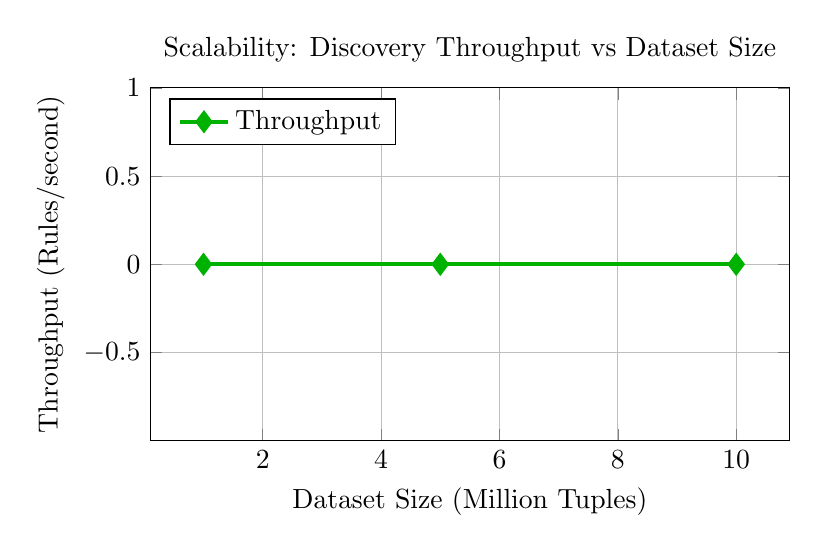
\begin{tikzpicture}
\begin{axis}[
    width=0.8\textwidth,
    height=0.5\textwidth,
    xlabel={Dataset Size (Million Tuples)},
    ylabel={Throughput (Rules/second)},
    title={Scalability: Discovery Throughput vs Dataset Size},
    grid=major,
    legend pos=north west,
    ymajorgrids=true,
    xmajorgrids=true,
    mark size=3pt,
]

% Throughput data
\addplot[
    color=green!70!black,
    mark=diamond*,
    line width=1.5pt,
] coordinates {
    (1.0,0.00)
    (5.0,0.00)
    (10.0,0.00)
};
\addlegendentry{Throughput}

\end{axis}
\end{tikzpicture}
